\documentclass[a4paper, twocolumn]{article}
\usepackage[utf8]{inputenc}
\usepackage[T1]{fontenc}
\usepackage[pdftex, hidelinks,
            pdftitle={WireGuard-go over VSOCK},
            pdfauthor={Guilherme Balena Versiani},
            pdfsubject={How WireGuard-go was adapted to work over VSOCK},
            pdfkeywords={wireguard,vsock,go}]{hyperref}

\usepackage{bm}
\usepackage{caption}
\usepackage{listings}
\usepackage{pdfpages}
\usepackage{booktabs}
\usepackage{mathtools}
\usepackage{blindtext}
\usepackage{algorithmic}
\usepackage{geometry}
\usepackage{graphicx}
\usepackage{courier}
\usepackage{acronym}
\usepackage{amssymb}
\usepackage{amsthm}
\usepackage{siunitx}
\usepackage{algorithm}
\usepackage{newpxtext, newpxmath}
\usepackage{xcolor}
\usepackage{listings}
\usepackage[capitalize, noabbrev]{cleveref}
\usepackage[activate={true, nocompatibility}, final,
            tracking=true, kerning=true, spacing=true,
            factor=1100, stretch=10, shrink=10]{microtype}

\DeclareCaptionFormat{modifiedlst}{\rule{\linewidth}{0.85pt}\\[-2.9pt]#1#2#3}
\captionsetup[lstlisting]{format =  modifiedlst,
labelfont=bf,singlelinecheck=off,labelsep=space}
\lstset{basicstyle=\footnotesize\ttfamily,
        breakatwhitespace = false,
        breaklines = true,
        keepspaces = true,
        language = C++,
        showspaces = false,
        showstringspaces = false,
        frame = tb,
        numbers = left,
        numbersep = 5pt,
        xleftmargin = 16pt,
        framexleftmargin = 16pt,
        belowskip = \bigskipamount,
        aboveskip = \bigskipamount,
        escapeinside={<@}{@>}}

\title{\vspace{-1.5em}\textbf{WireGuard-go over VSOCK}}
\author{{\textbf{Guilherme Balena Versiani}} \\
        {\href{mailto:guilherme.versiani@zerohash.com}
        {\texttt{<guilherme.versiani@zerohash.com>}}} \\
        {ZeroHash LLC}}

\begin{document}

\maketitle

\begin{@twocolumnfalse}
\begin{abstract}

WireGuard is a modern VPN protocol that was originally written in C. Due to
the increasing popularity of the Go programming language, the need for a Go
implementation of the protocol arose. In early 2018, WireGuard's creator
Jason Donenfeld announced on the WireGuard mailing list that he was working
on a new Go implementation of the protocol called WireGuard-go. The goal of
WireGuard-go was to provide a lightweight and efficient implementation of the
WireGuard protocol that could be easily integrated into various projects and
platforms.

The purpose of this paper is to provide an overview of the WireGuard-go usage
to provide AWS Nitro Enclave's networking over an AWS Elastic Kubernetes
Service (EKS) through VSOCK.\@

\end{abstract}
\end{@twocolumnfalse}

\section{Background}\label{sec:introduction}

AWS Nitro Enclaves provide a highly secure and isolated environment for running
sensitive workloads. However, due to their isolation, Nitro Enclaves do not
have network access by default~\cite{amazon_2023}. This can pose a challenge for
applications that require network connectivity, such as those running in
Kubernetes clusters. To address this challenge, we designed a WireGuard-go
extension that supports VSOCK to provide full network access to Nitro Enclaves.

\subsection{VSOCK}\label{sec:vsock}

VSOCK, also known as vSocket or VMware Socket Direct Path I/O, is a
socket-based communication mechanism that enables efficient and secure
communication between virtual machines (guests) and the
host~\cite{vmware_2023}. It was designed to overcome the limitations of
traditional networking protocols when it comes to performance, latency, and
scalability in virtualized environments. It provides a high-performance
communication channel that is optimized for virtualized environments and is
designed to avoid the overhead associated with traditional network protocols.
It was first introduced in the Linux kernel in 2013 by VMware, and since then
it has been used in their VMware ESXi hypervisors, VMware Fusion and VMware
Workstation products. It is also supported in some cloud-based VMware
offerings, such as VMware Cloud on AWS and VMware Cloud Director.
QEMU\cite{qemu_2023}, a popular open-source virtualization platform, and
OpenShift, a container platform that includes virtualization capabilities based
on KubeVirt~\cite{kubevirt_2023}, are other examples of systems using VSOCK.\@

The \texttt{vsock} module was integrated in the Linux Kernel
3.9~\cite{linuxarch_2012}, so it is typically available on most modern Linux
distributions. When loaded, applications can create \texttt{AF\_VSOCK} sockets
to communicate~\cite{manvsock_2023}. Each VM is assigned a unique CID (Context
ID) that is used to identify it on the vsock network, while the host has an
unique identifier (CID 2). Valid socket types are \texttt{SOCK\_STREAM} and
\texttt{SOCK\_DGRAM}.\  \texttt{SOCK\_STREAM} provides connection-oriented byte
streams with guaranteed, in-order delivery.\  \texttt{SOCK\_DGRAM} provides a
connectionless datagram packet service with best-effort delivery and
best-effort ordering. Availability of these socket types is dependent on the
underlying hypervisor. AWS Nitro Enclaves hypervisor in particular does not
support \texttt{SOCK\_DGRAM} socket type. Sockets are affected by live
migration of virtual machines. Connected \texttt{SOCK\_STREAM} sockets become
disconnected when the virtual machine migrates to a new host. Applications
must reconnect when this happens.

\subsection{WireGuard}\label{sec:wireguard}

Among the most popular Open Source VPN software, WireGuard is known for its
high performance and low resource usage. It has a smaller codebase compared to
other VPN solutions, which makes it faster and easier to audit. WireGuard is
also designed to use modern cryptography that is more efficient, resulting in
lower CPU usage and longer battery life on mobile devices. As a comparative,
the popular OpenVPN is generally considered to have a higher resource usage
compared to WireGuard. It requires more CPU cycles and memory to establish and
maintain VPN connections due to its more complex protocol and encryption
algorithms. StrongSwan, another popular Open Source VPN software, has also
higher resource usage compared to both WireGuard and
OpenVPN~\cite{vpnperf_2019}.\@ As of March 2023, there have been 1 CVE
attributed to WireGuard (for Windows), 56 CVEs attributed to OpenVPN, and 47
CVEs attributed to strongSwan. WireGuard uses a variety of cryptographic
primitives, including the Noise Protocol Framework, which provides a secure way
to establish a shared secret key between the two devices, and a combination of
modern encryption algorithms, such as ChaCha20, Poly1305, BLAKE2s, and
Curve25519.

Our approach leverages WireGuard-go~\cite{wggo_2023}, a Go implementation of
WireGuard, to enable secure connectivity between the Nitro Enclave and
Kubernetes. WireGuard-go was created to provide a high-performance, portable,
and easy-to-use implementation of the WireGuard protocol in the Go programming
language, with the goal of making it easier for developers to create and deploy
secure VPN solutions on a wide range of platforms and devices.

Unlike other VPN protocols, WireGuard explicitly supports UDP
only~\cite{wglimits_2015}, which enables it to operate efficiently and avoid
the problems associated with TCP.\@ However, when interfacing with VSOCK on AWS
Nitro Enclaves, there is no support for \texttt{SOCK\_DGRAM}. Because of that,
the WireGuard-go-vsock~\cite{wgvsock_2023} code creates an optimized
\texttt{SOCK\_STREAM} channel between the VSOCK peers, and over that, normal
WireGuard datagrams are exchanged. It also worth mentioning that due to address
differences, the CID formed by a 32-bit integer gets mapped to an IPv4 address
at the WireGuard-go stack, and the port, that is also another 32-bit integer,
gets mapped into a 16-bit port to match TCP/IP ports.

It is important to note that a WireGuard VPN between a Kubernetes container and
an Enclave does not necessarily mean that the Enclave has access to the local
network, as WireGuard uses TUN devices~\cite{tuntap_2023}. Instead, it relies
on IP packet forwarding based on routing rules and Network Address Translation
(NAT). The WireGuard VPN creates a secure tunnel between the Enclave and the
Kubernetes container only, and traffic between the Enclave and the outside
world is still subject to routing rules and other network configurations.

Establishing a VPN through VSOCK between a host and an AWS Nitro Enclave allows
for direct network communication between the host and the Enclave through
``cryptographic tunnels'', where all communication is encrypted and transmitted
through a virtual network interface (like \texttt{wg0}) transparently. This
interface can be seen as a secure point-to-point link between two devices, and
all traffic is directed to it. This setup does not require a proxy, which is
usually the approach offered by the AWS SDK.\@ The Amazon's \texttt{vsock-proxy}
requires adding a traffic forwarder at the Enclave side, alongside with the
Enclave app, and configuring client libraries to use the local traffic
forwarder~\cite{vsockproxy_2023}. The other drawback of using
\texttt{vsock-proxy} is that it requires launching one instance per remote
address of the server to be proxied. The VPN simplifies the setup of libraries,
as there is no need to configure an HTTP proxy in each, and management of the
system, because it doesn't require multiple proxies one per service, while
still maintain security by keeping the attack surface small constrained to the
WireGuard peers and networking set at both sides.

Another project adopting a similar approach is
\texttt{nitriding}~\cite{winter2022framework}, with the exception they don't
implement a VPN.\@ But the outcome is similar, as they claim:

\begin{quote}
Nitriding creates a TAP interface inside the enclave, allowing your application
to transparently access the Internet without having to worry about VSOCK,
port forwarding, or tunneling.
\end{quote}

In this approach, a peer-to-peer network link is established between the
Enclave and a controlling application, known as the Relay, rather than relying
on a traditional proxy setup. The Relay conveys container configurations ---
including IP address, DNS search parameters, and default gateway settings —--
back to the Enclave application, all while facilitating the establishment of a
peer-to-peer VPN via VSOCK\@. Unlike \texttt{nitriding}, the Relay possesses
the added capability of attesting the Enclave application's integrity before
permitting traffic to flow to or from it. This additional layer of security
significantly enhances the solution's robustness, rendering Enclave tampering
far less likely to occur.

\subsection{Kubernetes}\label{sec:kubernetes}

The Relay is hosted by an AWS EKS (Kubernetes) environment, and deployed using
regular manifests, except they contain a few Nitro Enclave extensions. These
extensions indicates to Kubernetes where the Pods should be allocated, case
there are managed EKS nodes without Enclaves support and self-managed ones in
the same cluster, and also enable the \texttt{/dev/nitro\_enclaves} device on
the running containers, so that they can launch/terminate Enclaves. In order to
be able to manage NAT and port forwarding for the Enclave, the Relay container
also has to have the \texttt{NET\_ADMIN} capability. 

\begin{figure}
  \centering
  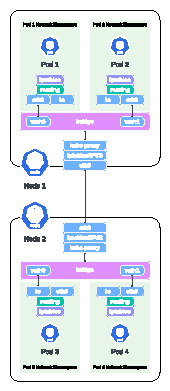
\includegraphics[height=14cm,keepaspectratio]{kubernetes-arch.pdf}
  \caption{Kubernetes networking.}\label{fig:k8s-arch1}
\end{figure}

One of the concerns that arise from the \texttt{NET\_ADMIN} enablement is that
firewall rules would conflict with \texttt{kube-proxy} or CNI.\@ But this is
not the case. Kubernetes provides network isolation to Pods through various
mechanisms implemented in the Linux kernel itself. Each Pod is assigned a
unique IP address within the Kubernetes cluster, and this is achieved through
the use of \textit{network namespaces}~\cite{critelli_2022}. Network namespaces
provide a way to isolate network resources such as interfaces, routes, and
firewall rules, as shown in figure~\ref{fig:k8s-arch1}.

When a container is launched within a Kubernetes Pod, the Kubernetes CNI
(Container Network Interface) plugin creates a new network namespace for the
Pod. A \textit{new} virtual network device called \texttt{lo} (loopback
device), which is similar to the one in the default network namespace except it
is isolated, is set at the namespace. It also creates a new pair of network
devices, a virtual Ethernet device called \texttt{veth} residing in the parent
namespace, and the other end residing in the new child network namespace,
usually \texttt{eth0}. In order for them to work, the CNI connects the
\texttt{veth} device to a bridge or a physical network interface in the parent
namespace, allowing the container to communicate with the outside world. In
addition, it can also use Linux's firewall (\texttt{iptables} or
\texttt{bpfilter}) to implement network policies at the Node level for the Pod.
These rules are invisible to the Pods except when they get \texttt{hostNetwork}
access.

Kubernetes also supports various network plugins that allow for different
network topologies and configurations, such as Cillium. These plugins are
responsible for implementing the network model of the cluster, and they can be
used to provide additional network isolation and security. Due to the usage of
network namespaces, none of these plugins conflict with the \texttt{iptables}
rules used by the Relay.

\subsection{Security}

The \texttt{NET\_ADMIN} capability allows a container to perform various
networking-related tasks that are otherwise restricted in a default container
configuration. Some of the threats associated with a container configured with
\texttt{NET\_ADMIN} capability include:

\begin{itemize}

\item \textbf{Network sniffing and eavesdropping.} A container with
\texttt{NET\_ADMIN} capability can be used to sniff network traffic passing
through the host system's network interfaces. Attackers can use this
capability to capture sensitive information, such as credentials and other
sensitive data, as it traverses the network. By design, Enclave's data in
transit is encrypted, which mitigates this risk for Enclave's
communication, but other services not properly secured can be compromised.

\item \textbf{Network injection and packet spoofing.} With \texttt{NET\_ADMIN}
capability, a container can inject or modify network packets as they traverse
the network. Attackers can use this capability to launch various network
attacks, such as man-in-the-middle attacks or packet spoofing attacks.

\item \textbf{Network enumeration and reconnaissance.} A container with
\texttt{NET\_ADMIN} capability can be used to scan the host system's network
interfaces and map out its topology. Attackers can use this capability to
identify potential targets and vulnerabilities within the network.

\item \textbf{Network DoS attacks.} With \texttt{NET\_ADMIN} capability, a
container can be used to launch various types of network-based
denial-of-service (DoS) attacks against the host system or other network
resources.

\end{itemize}

\begin{quote}
To configure WireGuard without granting \texttt{NET\_ADMIN} capabilities, one would use
gVisor's networking stack to handle the WireGuard setup within the container.\ 
gVisor can intercept the necessary system calls made by the container to set
up WireGuard interfaces, manage routes, and handle firewall rules. This way,
the container can perform WireGuard configuration tasks securely within its
isolated environment without requiring escalated privileges.
\end{quote}


On the other hand, the benefits may outweigh the risks:

\begin{itemize}

\item Enclave's data in transit is encrypted, so network sniffing risks are
mitigated.

\item Enclaves are attested before use, communication is immune to network
injection and packet spoofing.

\item Because of the above, network enumeration and reconnaissance doesn't
expose sensitive information about internal systems; at the same time Enclave's
network devices are isolated and cannot be enumerated from the Node.

\item As the network in question is private, DoS attacks are less likely to be
implemented without being rapidly identified.

\end{itemize}

In any case, it is recommended to implement other security measures such as
network segmentation and access control because non Enclave services don't
offer any of the isolation characteristics of the Enclave.

\section{Architecture}

\begin{figure*}
  \centering
  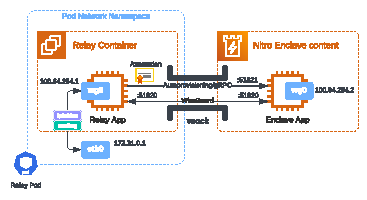
\includegraphics[width=\linewidth,keepaspectratio]{architecture.pdf}
  \caption{Enclave-Relay architecture.}\label{fig:arch1}
\end{figure*}

The AWS EKS cluster is created in a VPC.\@ By default, Pod networking is
provided by the Amazon VPC Container Network Interface (CNI) plugin, which can
be replaced by Cillium. Every CNI plugin allows Kubernetes Pods to have the
same IP address as they do on the VPC network. In this regard, there is nothing
special at Cillium when compared to Amazon CNI.\@

Linux kernel network namespaces are used to isolate network resources between
containers and Pods. When creating a Pod, several new namespaces are used for
isolation, including a network namespace to isolate the network of the
container. The network namespace provides a virtual network stack to the
container, which includes its own network interfaces, routing tables, and
\texttt{iptables} rules. This allows containers to have their own network namespace,
which is separate from the host network namespace and other containers.

Having the containers network isolated, the WireGuard peer implemented at the
Relay can make use of \texttt{iptables} to masquerade traffic from the Enclave and
ingress traffic to the Enclave by performing a destination NAT on the incoming
packets.

The syntax for these rules are presented in listings~\ref{lst:egress}
and~\ref{lst:ingress}.

\begin{minipage}{\linewidth}
\begin{lstlisting}[language=bash,caption={Enclave Egress},label={lst:egress}]
iptables -t nat -A POSTROUTING \
  -s 100.64.254.0/24 \
  -o eth0 \
  -j MASQUERADE
\end{lstlisting}
\end{minipage}

\begin{minipage}{\linewidth}
\begin{lstlisting}[language=bash,caption={Enclave Ingress},label={lst:ingress}]
iptables -t nat -A PREROUTING \
  -i eth0 -p tcp --dport 8080 \
  -j DNAT \
  --to-destination 100.64.254.2
\end{lstlisting}
\end{minipage}

The Enclave-Relay architecture is presented in figure~\ref{fig:arch1}. During
initialization, the Relay container uses \texttt{nitro-cli} to launch the
Enclave prior to starting its own Relay process. The Relay and the Enclave
applications start a WireGuard-go stack without any peer using random key
pairs. Then an auto provisioning step is performed at the next VSOCK port of
the WireGuard's one (by default the WireGuard port is 51820 so the auto
provisioning happens at the 51821), where the Relay acts as an initiator, and
the Enclave as a responder. The auto provisioning initiator connects to the
responder via VSOCK and offers all local network settings, including its
WireGuard-go public key and a \texttt{nonce} that is used at the attestation
document as a proof of authenticity of the Enclave. The Enclave configures its
local network, the loopback interface \texttt{lo}, the local IP of the
\texttt{wg0} interface, the default gateway is set to the Relay IP, and the DNS
settings are set as a copy from the Relay's one. The Enclave WireGuard-go stack
gets set with a peer entry corresponding to the Relay public key along with
other settings. As a response to the auto provisioning request, the Enclave
sends an attestation document containing the same \texttt{nonce} of the
request, and it's WireGuard-go's public key. The initiator receives the
attestation document and validates it; if valid, it sets up the Enclave's peer
at the WireGuard-go stack and the usual WireGuard protocol handshake starts,
assigning a shared key at both ends of the connection.

\subsection{Enclave Egress Traffic}

\begin{figure}
  \centering
  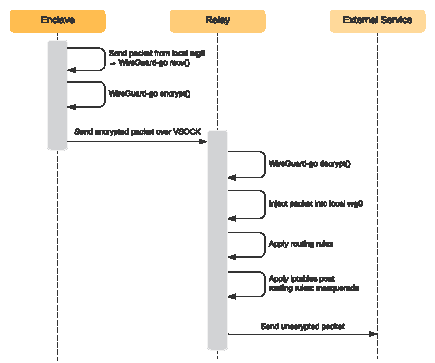
\includegraphics[width=\linewidth,keepaspectratio]{egress-sequence.pdf}
  \caption{Enclave Egress sequence.}\label{fig:egress-sequence1}
\end{figure}

The packet lifecycle from the perspective of the Enclave when it needs to
communicate with an external service is showed at the
figure~\ref{fig:egress-sequence1}, and described below:

\begin{enumerate}

\item The packet originates from the Enclave application hosted in an AWS Nitro
Enclave using the address assigned to \texttt{wg0} as the source address
according to the local routing rules, as the default gateway set at the
Enclave is the Relay address set at the WireGuard peer-to-peer connection.
The prepared WireGuard-go code is listening for packets on that \texttt{wg0}
TUN interface, so it intercepts the packet.

\item The WireGuard-go code uses the shared key established after the protocol
handshake to encrypt the packet.

\item The encrypted packet is sent over VSOCK, as initially provisioned by the
Relay.

\item The Relay application receives the encrypted packet from the VSOCK
interface, and delivers it to WireGuard-go, which decrypts the packet using the
shared key established during the protocol handshake.

\item The packet is injected into the local \texttt{wg0} interface, as if it
would have been received from the Enclave through a regular network
interface.

\item The local routing rules set at the Pod network namespace will apply,
meaning that the local default gateway will be used to dispatch the packet.

\item Then the local \texttt{iptables} rules also set at the Pod network namespace only
will apply. As it has been set to masquerade packets from the Enclave, the
source address switches to the Relay's local IP set at the \texttt{eth0}.

\item The Linux Kernel now sends the packet through the \texttt{eth0} network
namespace of the Pod, which is set by the Kubernetes CNI to bridge, VPN or
directly connect to the Node's \texttt{eth0} interface, reaching out to the
external service.

\end{enumerate}

\subsection{Enclave Ingress Traffic}

\begin{figure}
  \centering
  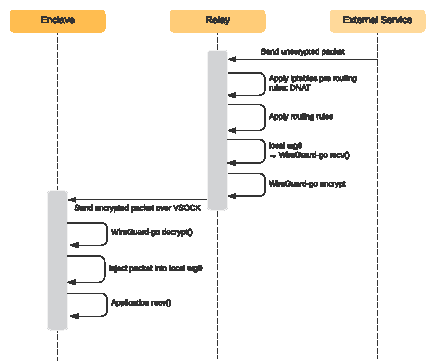
\includegraphics[width=\linewidth,keepaspectratio]{ingress-sequence.pdf}
  \caption{Enclave Ingress sequence.}\label{fig:ingress-sequence1}
\end{figure}

The packet lifecycle from the perspective of the Enclave when it receives data
from an external service is showed at the figure~\ref{fig:ingress-sequence1},
as described below:

\begin{enumerate}

\item According to the Kubernetes CNI, the packet is sent to the local
\texttt{eth0} of the Relay's Pod.

\item The \texttt{iptables} DNAT rules set at the Pod network namespace are applied, so
the destination address is set to the IP of the Enclave behind the VSOCK.\@

\item The routing rules set at the Pod network namespace are also applied,
which indicates that the interface to be used to dispatch the packet is the
local \texttt{wg0} interface.

\item The local TUN \texttt{wg0} interface is attached to the Relay's
WireGuard-go.

\item At the application level, WireGuard-go encrypts the packet with the
shared key exchanged during the protocol handshake.

\item The Relay sends the encrypted packet to the Enclave over VSOCK.\@

\item The WireGuard-go stack set at the Enclave side receives the packet and
decrypts it with the shared key exchanged during the protocol handshake.

\item The WireGuard-go then injects the unencrypted packet into the local
\texttt{wg0} TUN interface, as if it were just received from a regular network
interface.

\item As the destination address of the packet is the local IP set at the
\texttt{wg0}, the Linux Kernel then delivers the packet to the Enclave
application.

\end{enumerate}

\section{Conclusion}

This paper presented the solution for using WireGuard-go over VSOCK in an
Elastic Kubernetes Service (EKS) with support to AWS Nitro Enclaves. We
demonstrated that Kubernetes already provides network isolation so that
\texttt{iptables} commands do not interfere with it. The solution securely
connects Enclave-based applications with external networks using WireGuard
encrypted traffic. We showed how the implementation of WireGuard-go over VSOCK
provides a secure and efficient communication channel for Enclave-based
applications.

\nocite{*} % TODO: remove

\bibliographystyle{acm}
\bibliography{paper}

%\appendix
%\input{sections/appendices.tex}

\end{document}
